% ------------------------------------------------------------------------
% ------------------------------------------------------------------------
% Modelo UFSC para Trabalhos Academicos (tese de doutorado, dissertação de
% mestrado) utilizando a classe abntex2
%
% Autor: Nilton Aguiar dos Santos
% ------------------------------------------------------------------------
% ------------------------------------------------------------------------

\documentclass[
	% -- opções da classe memoir --
	12pt,				% tamanho da fonte
	%openright,			% capítulos começam em pág ímpar (insere página vazia caso preciso)
	oneside,			% para impressão no anverso. Oposto a twoside
	a4paper,			% tamanho do papel. 
	% -- opções da classe abntex2 --
	chapter=TITLE,		% títulos de capítulos convertidos em letras maiúsculas
	section=TITLE,		% títulos de seções convertidos em letras maiúsculas
	%subsection=TITLE,	% títulos de subseções convertidos em letras maiúsculas
	%subsubsection=TITLE,% títulos de subsubseções convertidos em letras maiúsculas
	% -- opções do pacote babel --
	english,			% idioma adicional para hifenização
	%french,				% idioma adicional para hifenização
	%spanish,			% idioma adicional para hifenização
	brazil				% o último idioma é o principal do documento
	]{abntex2}

\usepackage{Pacotes/UFMTThesis}

% ---
% Filtering and Mapping Bibliographies
% ---
% Pacotes de citações
% ---
\usepackage{csquotes}
\usepackage[backend = biber, style = abnt]{biblatex}
% FIXME Se desejar estilo numérico de citações,  comente a linha acima e descomente a linha a seguir.
% \usepackage[backend = biber, style = numeric-comp]{biblatex}

\setlength\bibitemsep{\baselineskip}
\DeclareFieldFormat{url}{Disponível~em:\addspace\url{#1}}
\NewBibliographyString{sineloco}
\NewBibliographyString{sinenomine}
\DefineBibliographyStrings{brazil}{%
	sineloco     = {\mkbibemph{S\adddot l\adddot}},
	sinenomine   = {\mkbibemph{s\adddot n\adddot}},
	andothers    = {\mkbibemph{et\addabbrvspace al\adddot}},
	in			 = {\mkbibemph{In:}}
}

\addbibresource{PosTextuais/Bibliografia.bib} % Seus arquivos de referências

% ---
\DeclareSourcemap{
	\maps[datatype=bibtex]{
		% remove fields that are always useless
		\map{
			\step[fieldset=abstract, null]
			\step[fieldset=pagetotal, null]
		}
		% remove URLs for types that are primarily printed
%		\map{
%			\pernottype{software}
%			\pernottype{online}
%			\pernottype{report}
%			\pernottype{techreport}
%			\pernottype{standard}
%			\pernottype{manual}
%			\pernottype{misc}
%			\step[fieldset=url, null]
%			\step[fieldset=urldate, null]
%		}
		\map{
			\pertype{inproceedings}
			% remove mostly redundant conference information
			\step[fieldset=venue, null]
			\step[fieldset=eventdate, null]
			\step[fieldset=eventtitle, null]
			% do not show ISBN for proceedings
			\step[fieldset=isbn, null]
			% Citavi bug
			\step[fieldset=volume, null]
		}
	}
}
% ---

% ---
% Informações de dados para CAPA e FOLHA DE ROSTO
% ---
% FIXME Substituir 'Nome completo do autor' pelo seu nome.
\autor{Nilton Aguiar dos Santos}
% FIXME Substituir 'Título do trabalho' pelo título da trabalho.
\titulo{DRD}
% FIXME Substituir 'Subtítulo (se houver)' pelo subtítulo da trabalho.  
% Caso não tenha substítulo, comente a linha a seguir.
\subtitulo{Uma aplicação de reconciliação de dados utilizando métodos de Lagrange}
% FIXME Substituir 'XXXXXX' pelo nome do seu
% orientador.
\orientador{Prof. Dr. João Gustavo Coelho Pena}
% FIXME Se for orientado por uma mulher, comente a linha acima e descomente a linha a seguir.
% \orientador[Orientadora]{Nome da orientadora, Dra.}
% FIXME Substituir 'XXXXXX' pelo nome do seu
% coorientador. Caso não tenha coorientador, comente a linha a seguir.
% \coorientador{Prof. XXXXXX, Dr.}
% FIXME Se for coorientado por uma mulher, comente a linha acima e descomente a linha a seguir.
% \coorientador[Coorientadora]{XXXXXX, Dra.}
% FIXME Substituir 'XXXXXX' pelo nome do Coordenador do 
% programa/curso.
% \coordenador{Prof. XXXXXX, Dr.}
% FIXME Se for coordenadora mulher, comente a linha acima e descomente a linha a seguir.
% \coordenador[Coordenadora]{Nome da Coordenadora, Dra.}
% FIXME Substituir '[ano da entrega]' pelo ano (ano) em que seu trabalho foi defendido.
\ano{2024}
% FIXME Substituir '[dia] de [mês] de [ano]' pela data em que ocorreu sua defesa.
\data{29 de Novembro de 2024}
% FIXME Substituir '[Cidade da defesa]' pela cidade em que ocorreu sua defesa.
\local{Cuiabá}
\instituicaosigla{UFMT}
\instituicao{Universidade Federal de Mato Grosso}
% FIXME Substituir 'Dissertação/Tese' pelo tipo de trabalho (Tese, Dissertação). 
\tipotrabalho{Trabalho de Conclusão de Curso}
% FIXME Substituir '[licenciado/bacharel] em [nome do título obtido]' pela grau adequado.
\formacao{Bacharel em Engenharia de Computação}
% FIXME Substituir '[licenciado/bacharel]' pelo nivel adequado.
\nivel{bacharel}
% FIXME Substituir 'Curso de Graduação em [XXXXXXXX]' pela curso adequado.
\programa{Engenharia de Computação}
% FIXME Substituir 'Campus XXXXXX ou Centro de XXXXXX' pelo campus ou centro adequado.
\centro{Campus de Várzea Grande}
\preambulo
{%
\imprimirtipotrabalho~do~\imprimirprograma~do~\imprimircentro~da~\imprimirinstituicao~para~a~obtenção~do~título~de~\imprimirformacao.
}
% ---

% ---
% Configurações de aparência do PDF final
% ---
% alterando o aspecto da cor azul
\definecolor{blue}{RGB}{41,5,195}
% informações do PDF
\makeatletter
\hypersetup{
     	%pagebackref=true,
		pdftitle={\@title}, 
		pdfauthor={\@author},
    	pdfsubject={\imprimirpreambulo},
	    pdfcreator={LaTeX with abnTeX2},
		pdfkeywords={ufmt, latex, abntex2}, 
		colorlinks=true,       		% false: boxed links; true: colored links
    	linkcolor=black,%blue,          	% color of internal links
    	citecolor=black,%blue,        		% color of links to bibliography
    	filecolor=black,%magenta,      		% color of file links
		urlcolor=black,%blue,
		bookmarksdepth=4
}
\makeatother

% Declaração das siglas
\siglalista{ABNT}{Associação Brasileira de Normas Técnicas}

% Declaração dos simbolos
\simbololista{C}{\ensuremath{C}}{Circunferência de um círculo}
\simbololista{pi}{\ensuremath{\pi}}{Número pi} 
\simbololista{r}{\ensuremath{r}}{Raio de um círculo}
\simbololista{A}{\ensuremath{A}}{Área de um círculo}

\makenoidxglossaries 
\makeindex

\begin{document}
\selectlanguage{brazil}
\frenchspacing 
\OnehalfSpacing

\imprimircapa

\imprimirfolhaderosto*

\begin{fichacatalografica}
	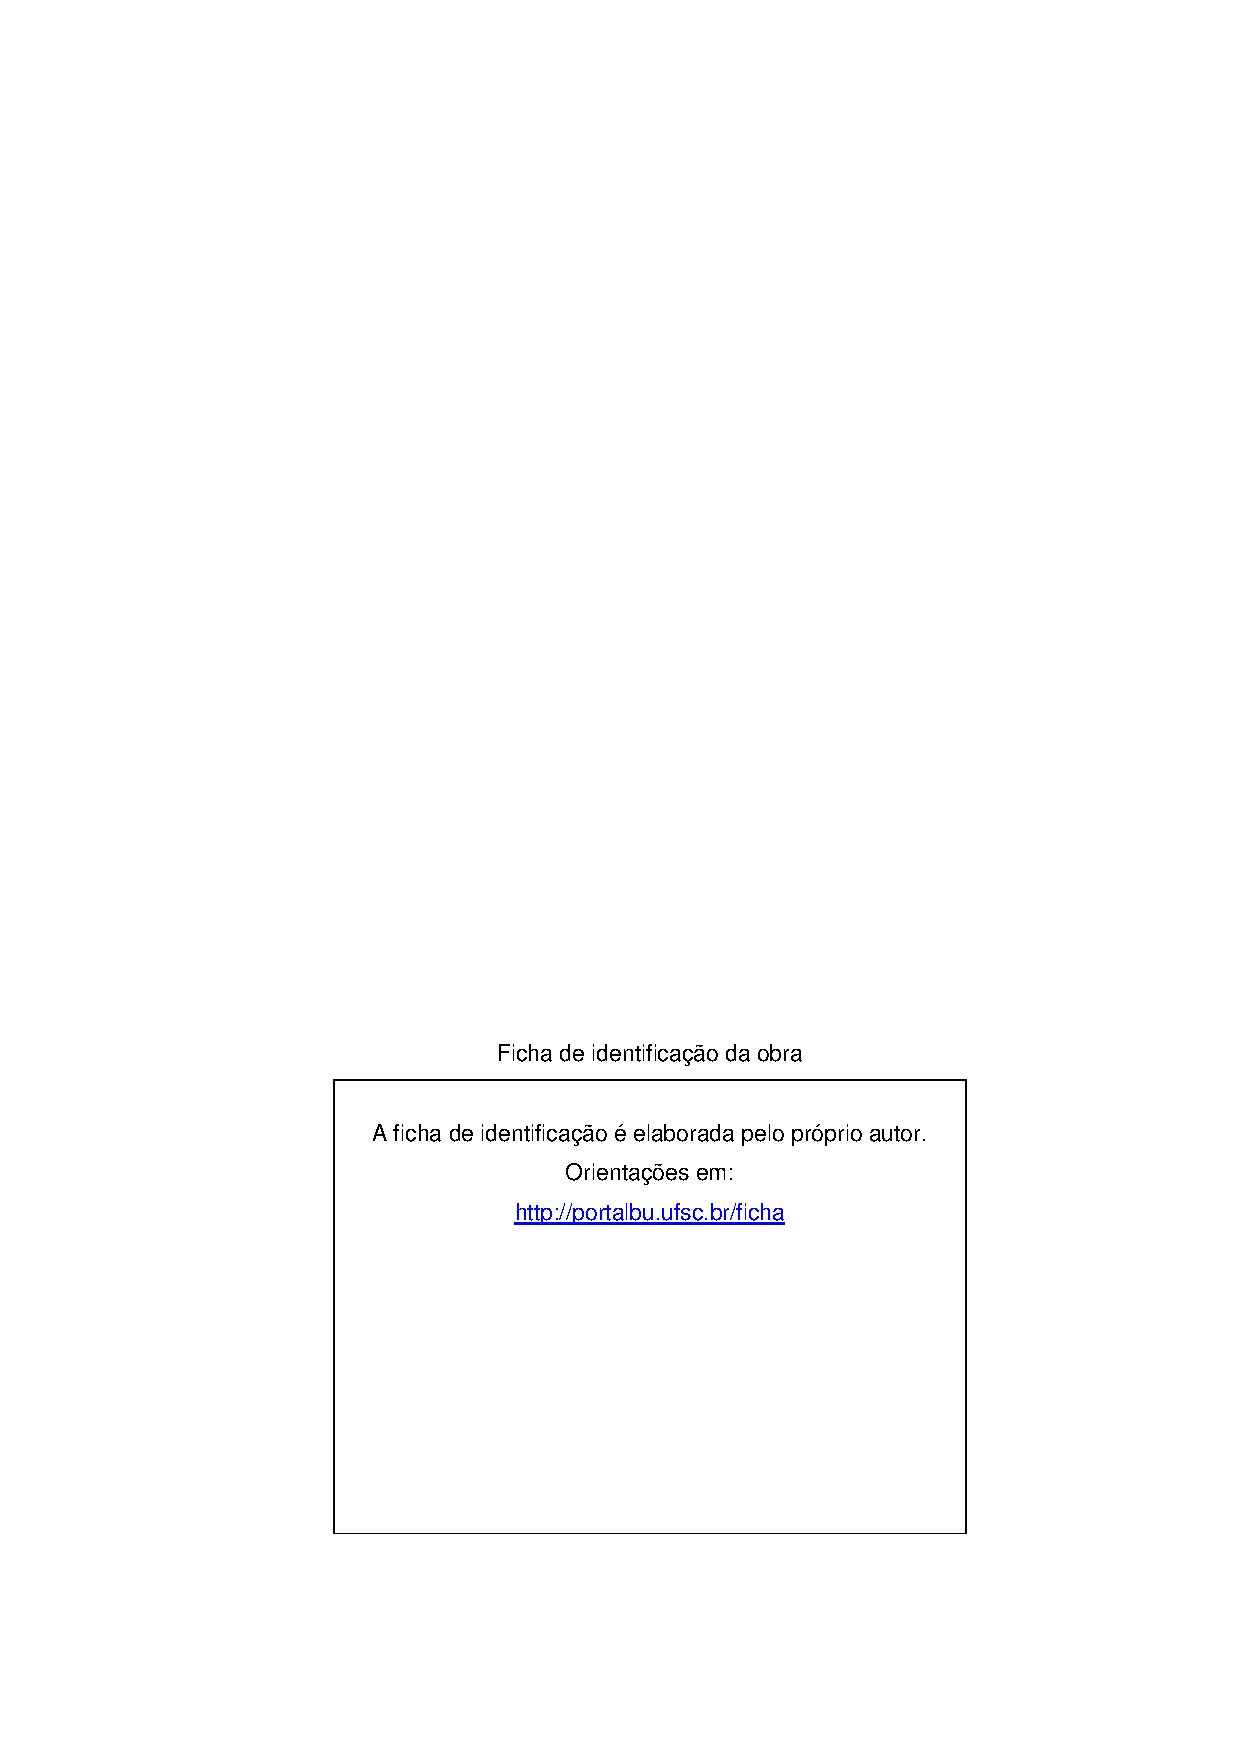
\includepdf{PreTextuais/Ficha_Catalografica.pdf}
\end{fichacatalografica}

\begin{folhadeaprovacao}
	\OnehalfSpacing
	\centering
	\imprimirautor\\%
	\vspace*{10pt}		
	\textbf{\imprimirtitulo}%
	\ifnotempty{\imprimirsubtitulo}{:~\imprimirsubtitulo}\\%
	%		\vspace*{31.5pt}%3\baselineskip
	\vspace*{\baselineskip}
	%\begin{minipage}{\textwidth}
	% ~do~\imprimirprograma~do~\imprimircentro~da~\imprimirinstituicao~para~a~obtenção~do~título~de~\imprimirformacao.
	Este~\imprimirtipotrabalho~foi julgado adequado para obtenção do Título de “\imprimirformacao” e aprovado em sua forma final pelo~\imprimirprograma. \\
		\vspace*{\baselineskip}
	\imprimirlocal, \imprimirdata. \\
	\vspace*{2\baselineskip}
	\assinatura{\OnehalfSpacing\imprimircoordenador \\ \imprimircoordenadorRotulo~do Curso}
	\vspace*{2\baselineskip}
	\textbf{Banca Examinadora:} \\
	\vspace*{\baselineskip}
	\assinatura{\OnehalfSpacing\imprimirorientador \\ \imprimirorientadorRotulo}
	%\end{minipage}%
	\vspace*{\baselineskip}
	\assinatura{Prof.(a) xxxx, Dr(a).\\
	Avaliador(a) \\
	Instituição xxxx}

	\vspace*{\baselineskip}
	\assinatura{Prof.(a) xxxx, Dr(a).\\
	Avaliador(a) \\
	Instituição xxxx}


\end{folhadeaprovacao}

\begin{dedicatoria}
    \vspace*{\fill}
    \noindent
    \begin{adjustwidth*}{}{5.5cm}     
        Aos meus pais, José Roberto dos Santos e Teresa de Jesus de Souza Aguiar, por cada sacrifício, por cada gesto de amor, por cada exemplo de dedicação. Aos meus irmãos por acreditaram em meu potencial e caminharam ao meu lado nesta jornada acadêmica. À minha namorada por ter me motivado a cada segundo do processo.
    \end{adjustwidth*}
\end{dedicatoria}

\begin{agradecimentos}
    Agradeço à Faculdade de Engenharia da Universidade Federal de Mato Grosso pela excelência acadêmica proporcionada, que enriqueceu meu conhecimento e habilidades. 
    
    Expresso minha gratidão à dedicada equipe de professores e funcionários, cujo comprometimento a frente de tantas dificuldades e complicações, não recuaram em oferecer um ensinamento completo a cada aluno, que contribuiu significativamente para o meu crescimento profissional. Esta instituição desempenhou um papel fundamental no meu desenvolvimento acadêmico, sendo um privilegiado ambiente de aprendizado.
    
    Agradeço ao professor João Gustavo Coelho Pena pela confiança, parceria, pela atenção e confiança, que possibilitou a construção desse trabalho. 
\end{agradecimentos}

\begin{epigrafe}
    \vspace*{\fill}
    \begin{flushright}
        \textit{``Não é o conhecimento, mas o ato de aprender.\\
        Não a posse, mas o ato de chegar lá\\
        Que garante o maior prazer''\\
        (Carl Friedrich Gauss)}
    \end{flushright}
\end{epigrafe}
% ---

\setlength{\absparsep}{18pt} % ajusta o espaçamento dos parágrafos do resumo
\begin{resumo}
    \SingleSpacing
    Neste trabalho de conclusão de curso, desenvolveu-se DRD (Dashboard of Data Reconciliation), um software online de análise, reconciliação e qualidade de dados utilizando técnicas de minimização de funções multivariáveis pelo método dos multiplicadores de Lagrange. A solução toma como prioridade uma abordagem baseada na web, oferecendo ao usuário a capacidade de realizar a análise e reconciliação de dados de forma remota e eficiente, com foco nos conceitos computacionais modernos afim dessa experiência ser a mais facilitada possível. Se utiliza durante todo o software a aplicação dos cálculos matemáticos e estatísticos voltados ao problema de análise, reconciliação e qualidade de dados. 
    
    Por meio da ferramenta é possível modelar todo um processo industrial e alimenta-lo com os dados oriundos da planta em questão e a partir disso analisar, reconciliar e verificar a qualidade dos dados em tempo real. O software é uma solução inovadora dado que não há um direto competidor para as funções oferecidas em um ambiente mais acessível e ágil no estado de Mato Grosso. Ao longo deste trabalho, o processo filosófico do desenvolvimento, os cálculos matemáticos, os conceitos estatísticos, computacionais e a lógica do software aplicado como solução são explicados de forma detalhada. Exemplos do código funcional e considerações finais sobre o trabalho realizado são apresentados nos últimos capítulos.
	
    \textbf{Palavras-chave}: Reconciliação de Dados. Análise de Qualidade de Dados. Desenvolvimento Web. Multiplicadores de Lagrange. Desenvolvimento de Software. Indústria 4.0.
\end{resumo}

% resumo em inglês
\begin{resumo}[Abstract]
    \SingleSpacing
    \begin{otherlanguage*}{english}
    In this undergraduate thesis, the development of DRD (Dashboard of Data Reconciliation) was undertaken, an online software for data analysis, reconciliation, and quality assessment using techniques of multivariable function minimization through the method of Lagrange multipliers. The solution prioritizes a web-based approach, providing users with the ability to remotely and efficiently perform data analysis and reconciliation, focusing on modern computational concepts to ensure a user-friendly experience. The software applies mathematical and statistical calculations throughout, specifically tailored to the problems of data analysis, reconciliation, and quality.

    Through this tool, it is possible to model an entire industrial process and feed it with data from the relevant plant, allowing real-time analysis, reconciliation, and quality verification. The software stands out as an innovative solution, as there is no direct competitor offering similar functions in a more accessible and agile environment in the state of Mato Grosso. This work details the philosophical process of development, mathematical calculations, statistical and computational concepts, and the logic of the software as an applied solution. Examples of functional code and final considerations about the work are presented in the last chapters.
    
    \textbf{Keywords}:  Data Reconciliation. Data Quality Analysis. Web Development. Lagrange Multipliers. Software Development. Industry 4.0.
    \end{otherlanguage*}
\end{resumo}

{
    \hypersetup{hidelinks}
    
    \pdfbookmark[0]{\listfigurename}{lof}
    \listoffigures*
    \cleardoublepage
    
    \pdfbookmark[0]{\listofquadrosname}{loq}
    \listofquadros*
    \cleardoublepage
    
    \pdfbookmark[0]{\listtablename}{lot}
    \listoftables*
    \cleardoublepage
        
    \imprimirlistadesiglas
    \imprimirlistadesimbolos
    
    \pdfbookmark[0]{\contentsname}{toc}
    \tableofcontents*
    \cleardoublepage
}

\textual

\chapter{Introdução} \label{Introducao}

O panorama atual sugere que o setor industrial brasileiro continua a crescer (Tomás Torezani, 2020) porém com ele deve seguir paralelamente um avanço tecnológico para que ela consiga aumentar o nível de produtividade dessas indústrias (Marcos Lisboa, 2021), dessa forma se origina o funcionalidade do trabalho de conclusão de curso DRD (Dashboard de Reconciliação de Dados), na qual ele unifica a área de análise de qualidade dos dados e a reconciliação desses mesmos com a tecnologia oriunda dos avanços tecnológicos na área de desenvolvimento web.

\section{Objetivos}

\subsection{\textit{Objetivo geral}}

Considerado a necessidade de inovação na área industrial e da união entre essas duas áreas, o objetivo deste trabalho é apresentar o desenvolvimento de um sistema online de reconciliação de dados utilizando métodos matemáticos criados por Lagrange.

\subsection{\textit{Objetivos específicos}}

Para alcançar o objetivo proposto neste trabalho, cuja finalidade é desenvolver uma ferramenta online de reconciliação de dados é necessário especificar os seguintes objetivos específicos:

a) Realizar a pesquisa de estado da arte da área de desenvolvimento de software para tal função.

b) Analisar e compreender as metodologias e algoritmos existentes na área de reconciliação de dados, destacando suas aplicações, vantagens e limitações. A pesquisa de estado da arte é crucial para identificar as tendências mais recentes, as melhores práticas e as lacunas existentes, proporcionando uma base sólida para o desenvolvimento da ferramenta online.

c) Selecionar e adaptar as tecnologias adequadas para a implementação da ferramenta online de reconciliação de dados. Isso envolverá a avaliação de linguagens de programação, frameworks e plataformas que melhor se adéquem aos requisitos específicos da aplicação, considerando aspectos como eficiência, escalabilidade e segurança.

d) Projetar a arquitetura da ferramenta, delineando os componentes principais, a interação entre eles e a lógica de funcionamento. A clareza na definição da arquitetura será essencial para garantir a eficácia operacional da ferramenta, bem como para facilitar futuras atualizações e expansões.

e) Desenvolver a ferramenta online de reconciliação de dados, implementando os algoritmos e funcionalidades identificados na pesquisa de estado da arte. Durante essa fase, é crucial garantir a usabilidade, a integridade dos dados e a eficiência do sistema, atendendo aos padrões de qualidade e performance esperados.

f) Realizar testes abrangentes para validar a eficácia e confiabilidade da ferramenta. Isso incluirá testes de integração, testes de segurança e simulações de casos práticos para verificar a capacidade da ferramenta em lidar com diferentes cenários e volumes de dados.

g) Elaborar uma documentação completa, abrangendo desde o processo de desenvolvimento até as instruções de uso da ferramenta. Uma documentação robusta e clara será essencial para facilitar a compreensão, manutenção e futuras implementações relacionadas à ferramenta de reconciliação de dados.

\section{Justificativa}

A ferramenta online de reconciliação de dados baseia-se na interseção entre a indústria e tecnologia da internet 4.0. Observa-se a necessidade premente de ferramentas especializadas que possam acompanhar e potencializar essa convergência, contribuindo para a eficiência operacional, qualidade dos processos industriais e aprimoramento da competitividade das empresas. A atual revolução industrial demanda soluções tecnológicas avançadas que permitam a integração e análise eficiente de dados em tempo real. A solução DRD torna-se crucial para manter a integridade das informações, garantindo a consistência e confiabilidade necessárias para operações industriais avançadas.

A utilização de uma ferramenta online de reconciliação de dados abre caminho para a otimização de processos, unificação com outras ferramentas, redução de erros, monitoramento em tempo real e, consequentemente, aumento da eficiência operacional. Isso não apenas reduz custos operacionais, mas também posiciona as empresas em um patamar competitivo mais vantajoso. E a integração dessa ferramenta com outras permite não apenas a reconciliação de dados, mas também a extração de insights valiosos para a tomada de decisões estratégicas. Essa sinergia contribui para a inovação contínua e a adaptação rápida às mudanças no ambiente industrial.

O desenvolvimento de uma ferramenta posiciona-se em consonância com as tendências globais de transformação digital e automação industrial. Isso não apenas fortalece a competitividade das empresas no mercado nacional, mas também as prepara para atuar de maneira efetiva em uma escala internacional. Em suma, diante do cenário tecnológico atual e das demandas evolutivas da indústria, a criação de uma ferramenta online de reconciliação de dados emerge como uma resposta estratégica para potencializar a interseção entre a Internet e o setor industrial, impulsionando a eficiência e a inovação nas práticas industriais contemporâneas.

\section{Estado da Arte}

Este trabalho está organizado da seguinte forma: (descrever)....

\section{Organização do Texto}

Este trabalho está organizado da seguinte forma: (descrever)....

%Sugestões para estrutura da monografia:

% \begin{enumerate}[label=(\alph*)]
%   \item Introdução
%   \item Referencial Teórico (ou Revisão Bibliográfica)
%   \item Materiais e Métodos (ou Metodologia)
%   \item Resultados e Discussões
%   \item Conclusão (ou Considerações Finais)
%   \item Referências
% \end{enumerate}
\chapter{Referencial Teórico} \label{RevisaoBibliografica}

\section{Reconciliação de Dados}
% Reconciliação de Dados
% ========================================================
% QUESTÃO:

\subsection{Definição}

A reconciliação de dados é uma prática de tratamento de dados em diversos campos da ciência e da engenharia, visando garantir a consistência e a precisão dos dados coletados a partir de diferentes fontes [REFERÊNCIA]. Em sua essência, a reconciliação de dados consiste no processo de comparar e corrigir dados divergentes ou inconsistentes, a fim de garantir que todas as informações disponíveis estejam alinhadas e concordantes. Esse processo é essencial em contextos nos quais múltiplas fontes de dados são utilizadas, como em sistemas industriais, processos químicos, redes de sensores e modelagem ambiental [REFERÊNCIA].

A reconciliação de dados envolve a aplicação de técnicas estatísticas e matemáticas para identificar e corrigir discrepâncias entre os dados observados e os valores esperados, com base em modelos e relações conhecidas [REFERÊNCIA]. Isso pode incluir a detecção e correção de erros sistemáticos ou aleatórios, a estimativa de valores ausentes e a harmonização de diferentes tipos de dados. Ao garantir a consistência e a confiabilidade dos dados, a reconciliação de dados permite uma análise mais precisa e uma tomada de decisão mais fundamentada em uma variedade de contextos aplicados [REFERÊNCIA].

Em suma, a reconciliação de dados desempenha um papel crucial na garantia da qualidade e integridade dos dados em diferentes áreas de aplicação. Ao alinhar e corrigir dados discrepantes, essa prática permite uma análise mais confiável e uma interpretação mais precisa dos fenômenos estudados, contribuindo assim para avanços significativos em diversos campos da ciência e da engenharia [REFERÊNCIA].

\subsection{Reconciliação de Dados no Âmbito Industrial}
% Reconciliação de Dados
% ========================================================
% QUESTÃO:

Já no começo da década de 60 se entendeu a importância do controle de processos químicos industriais por computadores utilizando técnicas matemáticas (KUEHN, 1961), dessa forma surge a área da computação voltada à reconciliação de dados, na qual há a comparação, validação e correção de informações coletadas em diferentes pontos do processo, afim de determinar a consistência dos dados, a qualidade dos mesmos ou até otimizar os processos (NARASIMHAN, 2000).

Ao longo das últimas décadas, os métodos de reconciliação de dados evoluíram significativamente, acompanhando os avanços tecnológicos e as demandas crescentes da indústria [REFERÊNCIA]. Com o advento de sistemas de automação mais avançados, sensores inteligentes e a proliferação de dispositivos conectados, a quantidade de dados gerados nas operações industriais aumentou drasticamente [REFERÊNCIA]. Nesse contexto, a reconciliação, análise e gestão de dados tornaram-se ferramentas indispensáveis para garantir a integridade e a confiabilidade das informações coletadas em tempo real[REFERÊNCIA].

Na era contemporânea, a reconciliação de dados desempenha um papel crucial na otimização dos processos industriais, contribuindo para a eficiência operacional e a redução e custos [REFERÊNCIA]. Sistemas avançados de reconciliação não apenas comparam e validam dados, mas também utilizam algoritmos sofisticados para identificar padrões, tendências e anomalias [REFERÊNCIA]. Essa capacidade analítica permite que as indústrias ajam proativamente, antecipando-se a problemas potenciais, otimizando a produção e melhorando a qualidade dos produtos finais [REFERÊNCIA].

\subsection{Reconciliação de Dados Pelo Método dos Multiplicadores de Lagrange}
% ---
% Reconciliação de dados utilizando o método dos multiplicadores de Lagrange
% ========================================================
% QUESTÃO: Será que é necessário uma maior explicação sobre esse tópico?

No sistema em questão a reconciliação de dados vai ser feita com a minimização de funções multivariáveis utilizando método dos multiplicadores de Lagrange, desenvolvida pelo matemático Joseph Louis Lagrange (1739-1813), que desenvolveu um método de encontrar o mínimo ou máximo de uma função multivariável sujeita a uma ou várias condições de restrição [REFERÊNCIA].

Nesse contexto, a aplicação do método dos multiplicadores de Lagrange destaca-se como uma abordagem matemática sofisticada e eficaz para resolver problemas complexos de reconciliação de dados [REFERÊNCIA]. A técnica proporciona uma estrutura robusta para lidar com situações em que é necessário otimizar uma função multivariável sujeita a restrições específicas. Ao utilizar os multiplicadores de Lagrange, o sistema ganha a capacidade de encontrar soluções que atendam simultaneamente às condições impostas, proporcionando uma reconciliação precisa e eficiente dos dados envolvidos [REFERÊNCIA]. Essa metodologia, fundamentada em princípios matemáticos sólidos, contribui para aprimorar a qualidade e a confiabilidade dos resultados obtidos, na qual a torna uma ferramenta valiosa para a solução proposta no trabalho [REFERÊNCIA].

\section{Desenvolvimento de um \textit{Software Online}}
% Desenvolvimento de uma ferramenta online
% ========================================================
% QUESTÃO: 

\subsection{Desenvolvimento Front-End}

A interface de usuário de um \textit{software}, também denominada de \textit{front-end}, desempenha um papel crucial no desenvolvimento de sistemas modernos [REFERÊNCIA]. É responsável por criar a experiência do usuário, tornando a interação com o software intuitiva, eficiente e agradável. Compreende todos os elementos visíveis e interativos de uma aplicação, como botões, menus, formulários e layouts, que são projetados e desenvolvidos para fornecer uma interface acessível e funcional aos usuários [REFERÊNCIA].

As principais tecnologias aplicadas a essa área dentro do desenvolvimento \textit{web} são linguagens de programação como HTML, CSS, JavaScript e TypeScript [REFERÊNCIA]. Essas tecnologias permitem aos desenvolvedores criar interfaces de usuário dinâmicas e responsivas, capazes de se adaptar a diferentes dispositivos e tamanhos de tela. Além disso, o \textit{front-end} envolve a utilização de \textit{frameworks}, \textit{runtimes} e bibliotecas importantes e poderosas, como React, Angular e Vue.js, que possibilitando um desenvolvimento rápido e eficiente de interfaces de usuário modernas [REFERÊNCIA]. Desta forma, o \textit{front-end} é uma parte essencial do processo de desenvolvimento de \textit{software}, desempenhando um papel fundamental na criação de sistemas interativos e centrados na experiência usuário [REFERÊNCIA].

\subsection{Desenvolvimento Back-End}

Muitas vezes referido com oa parte não visível ou o "cérebro" por trás de uma aplicação, o \textit{back-end} é igualmente crucial para o funcionamento de sistemas modernos [REFERÊNCIA]. Enquanto o \textit{front-end} é responsável pela parte visual e interativa da aplicação, o \textit{back-end} lida com a lógica de negócios, o armazenamento de dados e a comunicação com o servidor. Isso inclui operações como autenticação de usuários, processamento de dados, gerenciamento de sessões e acesso a banco de dados [REFERÊNCIA].

As tecnologias empregadas no \textit{back-end} são diversas, incluido linguagens de programação como Python, Ruby, Java, PHP e Node.js. Estas linguagens são utilizadas em conjunto com \textit{frameworks} e bibliotecas específicas para o desenvolvimento \textit{web}, como Django, Ruby on Rails, Spring, Laravel e Express.js [REFERÊNCIA]. O \textit{back-end} também envolve a criação de APIs (Interfaces de Programação de Aplicativos) para permitir a comunicação eficiente entre o \textit{front-end}, outros sistemas e o banco de dados. Desta forma, o \textit{back-end} é responsável por garantir que a aplicação web seja funcional, segura e capaz de processar grandes volumes de dados, desempenhando um papel crucial no sucesso de sistemas web modernos [REFERÊNCIA].

\subsection{Desenvolvimento de Banco de Dados}

No contexto do desenvolvimento de sistemas \textit{web}, o banco de dados desempenha um papel fundamental na organização e armazenamento de dados utilizados pela aplicação [REFERÊNCIA]. Ele oferece uma estrutura organizada e eficiente para armazenar informações de forma persistente, garantindo que os dados sejam recuperados de maneira rápida e precisa quando necessário. O banco de dados é responsável por gerenciar grandes volumes de dados, lidar com transações complexas e garantir a integridade e a segurança das informações armazenadas [REFERÊNCIA].

Existem diversos tipos de bancos de dados, cada um com suas características e funcionalidades específicas. Os bancos de dados relacionais, como MySQL, PostgreSQL e SQL Server, utilizam tabelas para organizar os dados em linhas e colunas, facilitando consultas complexas e garantindo a consistência dos dados por meio de relações definidas [REFERÊNCIA]. Por outro lado, os bancos de dados NoSQL, como MongoDB e Cassandra, oferecem uma abordagem mais flexível e escalável para o armazenamento de dados não estruturados, como documentos, gráficos e dados em tempo real [REFERÊNCIA].

Além disso, o banco de dados é essencial para a integridade e a consistência dos dados em uma aplicação web [REFERÊNCIA]. Ele permite que os desenvolvedores armazenem e recuperem informações de forma eficiente, garantindo que os dados sejam sempre precisos e atualizados. Por meio de consultas e transações, o banco de dados fornece uma camada de abstração entre a aplicação e os dados subjacentes, facilitando o acesso e a manipulação dos dados de forma segura e eficaz [REFERÊNCIA]. Desta forma, o banco de dados é um componente essencial do desenvolvimento de sistemas \textit{web}, garantindo que as informações sejam armazenadas e gerenciadas de maneira confiável e eficiente [REFERÊNCIA].

\subsection{Servidor}

Na arquitetura de sistemas web, o servidor desempenha um papel central na comunicação entre o cliente e o \textit{back-end}. Ele é responsável por receber as requisições dos clientes, processá-las e fornecer as respostas adequadas [REFERÊNCIA]. Além disso, o servidor também gerencia o armazenamento e o acesso aos dados, garantindo que as informações sejam entregues de forma rápida e segura [REFERÊNCIA].

As tecnologias utilizadas na área de servidor variam dependendo das necessidades específicas do projeto, mas geralmente incluem sistemas operacionais como Linux ou Windows Server, juntamente com servidores web como Apache, Nginx ou Microsoft IIS [REFERÊNCIA]. Além disso, frameworks e tecnologias como Docker, Kubernetes e AWS são frequentemente empregados para facilitar a implantação e o gerenciamento de servidores em escala. Em suma, a área de servidor é fundamental para o funcionamento eficiente e confiável de sistemas web, garantindo a entrega de conteúdo e serviços de forma rápida, segura e escalável [REFERÊNCIA].

\section{A Sinergia Entre a Indústria e a Internet}
% A sinergia entre a indústria e a internet
% ========================================================
% QUESTÃO: 

O panorama atual de avanço da internet e a convergência entre a internet e o setor industrial representam um arco significativo na era da Engenharia de Computação [REFERÊNCIA]. Este fenômeno transformador tem sido impulsionado pela fusão das tecnologias da informação com os processos industriais, dando origem a conceitos como Indústria 4.0. 

No âmbito desta ferramenta é aplicado a intersecção dessas duas esferas, onde os conceitos de práticas industriais, reconciliação, análise e qualidade de dados se integram à internet na qual é extraído deles o seu maior forte, como uma maior integralidade com outros sistemas por meio de APIs (interfaces de programação de aplicativos), melhor interatividade entre os elementos do sistema, promovendo uma comunicação mais dinâmica e eficaz, aumento da eficiência operacional e facilidade na gestão de processos [REFERÊNCIA]. Essa sinergia possibilita a criação de ecossistemas industriais mais conectados nos quais os dados relevantes podem ser tratados de forma segura e eficiente. [REFERÊNCIA].

O horizonte atual, delineado pelos recentes avanços tecnológicos e inovações sustenta a perspectiva otimista que as indústrias estão destinadas a experimentar um crescimento substancial no país [REFERÊNCIA]. A convergência entre a internet e o setor industrial, representa um catalisador significativo para a modernização e eficiência operacional. A integração de práticas avançadas de desenvolvimento de soluções voltadas a usabilidade e ambiente de desenvolvimento com controle computacional, como a reconciliação de dados e análise preditiva, impulsiona a qualidade e consistência dos processos produtivos [REFERÊNCIA].

Além disso, a aplicação da internet nas práticas industriais não só fortalece a competitividade das empresas mas também desempenha um papel crucial na expansão econômica do país [REFERÊNCIA]. A capacidade de adotar tecnologias inovadoras como a automação avançada, coloca as indústrias em uma posição estratégica para atender às crescentes demandas do mercado e elevar a produtividade [REFERÊNCIA]. Nesse sentido é plausível afirmar que diante do atual cenário tecnológico e das tendências emergentes, é indubitável a necessidade e importância da ferramenta desenvolvida nesse trabalho [REFERÊNCIA].
\chapter{Metodologia} \label{metodologia}

\section{Sessão 1}
% 
% ========================================================
% QUESTÃO:

Vivamus vitae arcu ullamcorper, eleifend leo vel, aliquet orci. Aenean pellentesque turpis quis mi vehicula bibendum. In tempor leo nunc, eu pellentesque purus euismod ac. Proin id massa libero. Duis ligula libero, scelerisque id diam sit amet, mollis pharetra urna. Sed vehicula nibh et metus viverra fermentum. Pellentesque tortor sem, elementum sit amet nunc ac, dapibus vulputate tellus. Vestibulum eleifend a lorem finibus euismod. Nulla vulputate odio quis velit congue eleifend ut quis quam.


\subsection{Subsessão 1}

Maecenas sit amet tortor neque. Nunc et tristique justo. Pellentesque eget scelerisque eros, vitae aliquet tortor. Aliquam ut tortor tempor, euismod massa in, interdum nisi. Aliquam congue congue libero, a faucibus magna cursus id. Aenean ut diam sit amet dolor tempor placerat ut a ex. Donec egestas est at nulla ultricies, quis mollis tortor ultricies. Sed et consequat enim. Nam non consectetur metus. Cras magna sem, laoreet gravida mauris id, sollicitudin tristique libero. Mauris sodales vel nisl ac vestibulum.

\clearpage

\chapter{Resultados} \label{resultado}

\section{Sessão 1}
% 
% ========================================================
% QUESTÃO:

Vivamus vitae arcu ullamcorper, eleifend leo vel, aliquet orci. Aenean pellentesque turpis quis mi vehicula bibendum. In tempor leo nunc, eu pellentesque purus euismod ac. Proin id massa libero. Duis ligula libero, scelerisque id diam sit amet, mollis pharetra urna. Sed vehicula nibh et metus viverra fermentum. Pellentesque tortor sem, elementum sit amet nunc ac, dapibus vulputate tellus. Vestibulum eleifend a lorem finibus euismod. Nulla vulputate odio quis velit congue eleifend ut quis quam.


\subsection{Subsessão 1}

Maecenas sit amet tortor neque. Nunc et tristique justo. Pellentesque eget scelerisque eros, vitae aliquet tortor. Aliquam ut tortor tempor, euismod massa in, interdum nisi. Aliquam congue congue libero, a faucibus magna cursus id. Aenean ut diam sit amet dolor tempor placerat ut a ex. Donec egestas est at nulla ultricies, quis mollis tortor ultricies. Sed et consequat enim. Nam non consectetur metus. Cras magna sem, laoreet gravida mauris id, sollicitudin tristique libero. Mauris sodales vel nisl ac vestibulum.

\clearpage

%\chapter{Considerações Finais} \label{consideracoes}

%%====== Section ========%
\chapter{Conclusão e Trabalhos Futuros}\label{conclusao}
\section{Reconciliação de Dados no Âmbito Industrial}
% Reconciliação de Dados
% ========================================================
% QUESTÃO:

Já no começo da década de 60 se entendeu a importância do controle de processos químicos industriais por computadores utilizando técnicas matemáticas (KUEHN, 1961), dessa forma surge a área da computação voltada à reconciliação de dados, na qual há a comparação, validação e correção de informações coletadas em diferentes pontos do processo, afim de determinar a consistência dos dados, a qualidade dos mesmos ou até otimizar os processos (NARASIMHAN, 2000).


\begingroup
    \SingleSpacing\printbibliography[title=REFERÊNCIAS]
\endgroup

\begin{apendicesenv} 
    %-------------------------------------------------------------
%---------------------- Apêndices ----------------------------
%-------------------------------------------------------------

\begin{apendicesenv}
%\partapendices  % Indica o início dos Apendices
\chapter{Informações para complementar o texto}

Note que os Apêndices são dedicados aos textos ou \textbf{documentação elaborados pelo próprio autor} que complemente  a  argumentação  textual  (códigos,  reportagens,  relatórios  etc.).

\lipsum[8]



\end{apendicesenv}
\end{apendicesenv}

\begin{anexosenv}
    % ----------------------------------------------------------
\chapter{Descrição}
% ----------------------------------------------------------

São documentos não elaborados pelo autor que servem como fundamentação (mapas, leis, estatutos). Deve ser precedido da palavra ANEXO, identificada por letras maiúsculas consecutivas, travessão e pelo respectivo título. Utilizam-se letras maiúsculas dobradas quando esgotadas as letras do alfabeto. 

\end{anexosenv}
\end{document}